\documentclass[conference]{IEEEtran}
\IEEEoverridecommandlockouts
\usepackage{graphicx}
\usepackage[colorlinks = true,
            linkcolor = black,
            urlcolor  = blue,
            citecolor = black,
            anchorcolor = blue]{hyperref}
\usepackage{amsmath,amssymb,amsfonts, mathtools}
\usepackage{algorithmic}
\usepackage{textcomp}
\usepackage{lipsum}                     
\usepackage{xargs}                      
\usepackage[pdftex,dvipsnames, table]{xcolor}  
\usepackage[table]{xcolor}
\usepackage{float}
\usepackage{subcaption}
\usepackage{stfloats}
\usepackage{bbm}
\usepackage[
backend=biber,
style=numeric,
sorting=ynt
]{biblatex}
\addbibresource[]{misc/references.bib}

\rowcolors{2}{gray!10}{white}

\newcommand{\titlecol}{\cellcolor{gray!30}}

% 
\usepackage[colorinlistoftodos,prependcaption,textsize=tiny]{todonotes}
\newcommandx{\unfinished}[2][1=]{\todo[linecolor=red,backgroundcolor=red!25,bordercolor=red,#1]{#2}}
\newcommandx{\change}[2][1=]{\todo[linecolor=blue,backgroundcolor=blue!25,bordercolor=blue,#1]{#2}}
\newcommandx{\info}[2][1=]{\todo[linecolor=OliveGreen,backgroundcolor=OliveGreen!25,bordercolor=OliveGreen,#1]{#2}}
\newcommandx{\improvement}[2][1=]{\todo[linecolor=Plum,backgroundcolor=Plum!25,bordercolor=Plum,#1]{#2}}
\newcommandx{\thiswillnotshow}[2][1=]{\todo[disable,#1]{#2}}

\begin{document}
\title{Image Analysis\\
{\footnotesize Optimization and Data Analytics mini-project}}

\author{\IEEEauthorblockN{Morten Lyng Rosenquist}
\IEEEauthorblockA{\textit{Faculty of Technical Sciences} \\
\textit{Aarhus University}\\
Aarhus, Denmark \\
201706031}
}

\maketitle

\begin{abstract}
This paper analyze the Image Classification problem for two different data sets. The classifiers used are Nearest Class Centroid, Nearest Sub-Class Centroid, Nearest Neighbor, Perceptron using Backpropagation and Perceptron using MSE. The classification is performed on the sets with full features and the sets having their features reduced to two utilizing PCA. It is seen that the methods vary in performance with respect to training time and testing accuracy.  
\end{abstract}

\begin{IEEEkeywords}
classification, orl, mnist, pca, data analytics
\end{IEEEkeywords}

\section{Introduction}
This thesis will analyze the Image Classification problem. Utilizing only supervised learning algorithms This revolves around training a classification model with train images and thereafter being able predict correct classes for test images. The computer doesn't see the physical images as humans will, instead it sees a vector or matrix of pixels. The used classification models is described in the following sections.     

\subsection{Nearest Centroid}
Nearest Centroid, also called Nearest Prototype, calculates the centroids of each class and then predicts an observation to a class whose mean is the closest. Given a set of N samples, where each sample is represented by a vector $\mathbf{x}_i\in\mathbbm{R}^D$ and the corresponding labels are denoted as $l_i$. The centroids are denoted as $\mathbf{\mu}_k, k=1,...,K$ where $K$ is the amount of classes. Then during training the centroids are defined\cite{ai-course-notes}: 

\begin{equation}
    \mathbf{\mu}_k = \frac{1}{N_k} \sum_{i,l_i=k}{\mathbf{x}_i}, k=1,...,K, 
\end{equation}

Having calculated the centroids, a new observation $\mathbf{x}_*$ can be calculated based on the minimal distance from $\mathbf{\mu}_k$: 

\begin{equation}
    d(\mathbf{x}_*, \mathbf{\mu}_k) = ||\mathbf{x}_*-\mathbf{\mu}_k||^2_2
\end{equation}

\subsection{Nearest sub-class Centroid}
Nearest sub-class centroid is similar to the Nearest Centroid. It introduces a new sub-class element, that divides each class in a set amount of subclasses. Then during training the centroids of the subclasses are calculated. During predictions an observation is classified to the class which subclass it had the minimal distance. Given a set of N samples, where each sample is represented by a vector $\mathbf{x}_i\in\mathbbm{R}^D$ and the corresponding labels are denoted as $l_i$. Having a sub classes $m$ of class $c_k$ the centroids of each class can then be calculated\cite{ai-course-notes}: 

\begin{equation}
    \mathbf{\mu}_{km} = \frac{1}{N_{km}} \sum_{i,l_i=k, q_i=m}{\mathbf{x}_i}, k=1,...,K,
\end{equation}

The subclass label of vector $\mathbf{x}_i$ is $q_i$ and $N_{km}$ is the amount of samples of class $c_k$ composing subclass m. Classification on observations can then be done based on distance similar to the Nearest Centroid: 

\begin{equation}
    d(\mathbf{x}_*, \mathbf{\mu}_{km}) = ||\mathbf{x}_*-\mathbf{\mu}_{km}||^2_2
\end{equation}

\subsection{Nearest Neighbor}
The Nearest Neighbor schema stores the training data and classifies observations based on which training data samples they are closest to. The amount of neighbors to specify is highly dependent on the data set. A high amount of neighbors reduces the effect of bad samples and noise\cite{nearest-neighbor}. Meanwhile a low amount of neighbors leads to spurious classifications of possible outliers. 

\subsection{Perceptron using Backpropagation or MSE}
Perceptron is a (binary) linear classifier that decides if an observation is in a class or not. As an example looking at only two classes $c_1$ and $c_2$. Given a weight vector $\mathbf{w}$ and a input vector $\mathbf{x}\in\mathbbm{R}^D$ then a linear discrimination function g is: 

\begin{equation}
    g(\mathbf{x})=\mathbf{x}^Tx + w_0 = \sum_{d=1}^D{w_dx_d+w_0}
\end{equation}

$x_0$ is called the bias. The class decision of $\mathbf{x}$ is then dependent on the result of $g(\mathbf{x})$: 

\begin{equation}
    l_i=
    \begin{cases}
        c_1& \text{if $g(x)>0$} \\
        c_2& \text{if $g(x)<0$}  \\
        c_1 \lor c_2& \text{if $g(x)=0$}
    \end{cases}
\end{equation}

The weights are updated after each sample: 

\begin{equation}
    \mathbf{w}(t+1) = \mathbf{w}(t) - \eta(t) {\Delta} J_p = \mathbf{x}(t) + \eta(t) \sum_{\mathbf{x}_i \in X}{l_i \mathbf{x}_i}
\end{equation}

Where $\eta(t)$ is the learning rate that is either constant during all samples or are being according to a certain algorithm. If the learning rate is to high the classifier will converge to fast and the decision boundaries will be incorrect. Otherwise if it's to low the classifier will be slow. $\Delta J_p$ is the gradient of our optimization problem. As for utilizing this classifier for a problem with more than two classes we need to combine multiple binary classifiers. One option is the one-versus-all. If there is K classes then we need K binary classifiers. First one that determines if one class is different from the others, and a second one that determines if the second class is different from the others, and so on. This utilizes backpropagation by updating $\mathbf{w}$ such that it will be more fit to handle a similar input the next time\cite{ai-course-notes}.     

Instead of utilizing backpropagation the Minimum Squared Error can be used. The goal is still to update $\mathbf{w}$ as optimal as possible. This is done by minimizing an error vector $\mathbf{e}$:

\begin{equation}
    \mathbf{e} = \mathbf{X}^T \mathbf{w} - \mathbf{b}
\end{equation}

Where X is a matrix with columns containing the training vectors and $\mathbf{b}$ is vector with the target values. Solving the optimization problem leads to\cite{ai-course-notes}: 


\begin{equation}
    \mathbf{w} = (\mathbf{X} \mathbf{X})^{-1} \mathbf{X} \mathbf{b} = \mathbf{X}^\dagger \mathbf{b}
\end{equation}

The backpropagation solution fits well when clear decision boundaries can be drawn between the classes. If that is not the case utilizing Minimum Square Error can be more beneficial. 

\subsection{Principal component analysis}
There is advantages and disadvantages in reducing the dimensions of the data. It makes it easier to visualize the data. Having the feature reduction as a preprocessing step the time of training and testing classifiers will reduce. As all data can not be covered in the reduced dimensions it will also result in reduced accuracy when performing classification. The goal in reducing features is keeping it uncorrelated, meaning it should be possible to still differ which class each sample belongs to. PCA works by the first dimension having the largest possible variance. Then remembering the first dimension each succeeding dimension is also to have the largest possible variance\cite{ai-course-notes}.  

\section{Databases}
The datasets that are analyzed in this paper are MNIST and ORL. 

\subsection{ORL}
The ORL data set contains 400 vectorized images. The images are of size 40x30 and depict a persons face in an upright position in a frontal view\cite{orl_images}. There is 10 images of 40 different persons. Examples of the images can be seen on Figure \ref{fig:orl-images-raw}.

\begin{figure}[htbp]
    \centering
    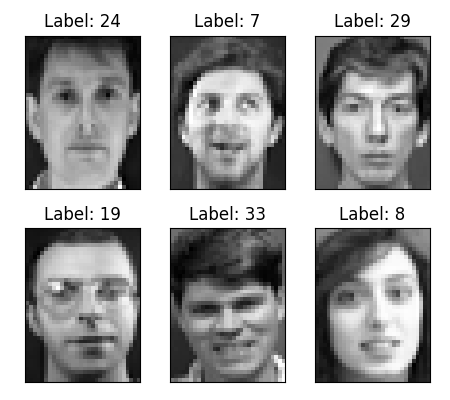
\includegraphics[width=0.7\columnwidth]{../source/orl/pictures/image-before-pca.png}
    \caption{ORL example images}
    \label{fig:orl-images-raw}
\end{figure}

\subsection{MNIST}
The MNIST dataset is larger with 70,000 vectorized images. The images depict handwritten digits and are of size 28x28. Differing from the ORL data set, the set is already split in training and test data. Leading to 60,000 images for training and 10,000 for testing. Examples from the MNIST data set can be seen on Figure \ref{fig:mnist-images-raw}.  

\begin{figure}[htbp]
    \centering
    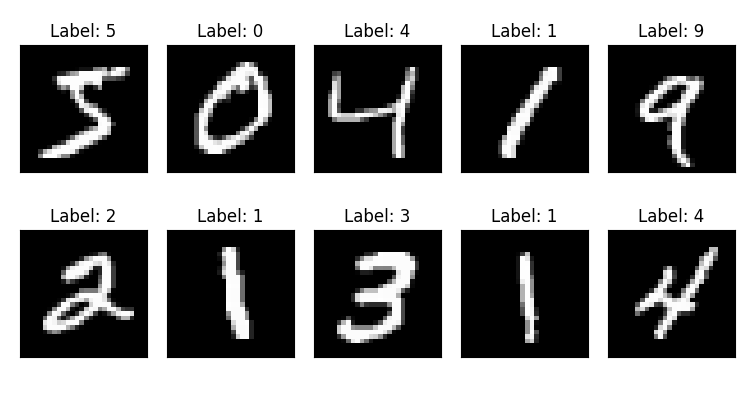
\includegraphics[width=0.7\columnwidth]{../source/mnist/pictures/image-before-pca.png}
    \caption{MNIST example images}
    \label{fig:mnist-images-raw}
\end{figure}

\section{Methods}
The classification and visualization of the data is implemented in python and the source code can be found on \href{https://github.com/mlRosenquist/oda-project-assignment/tree/master/source}{github} and in the attached zip folder. The primary packages used are \href{https://scikit-learn.org/stable/index.html}{sklearn} for data analysis and classification and \href{https://matplotlib.org/}{matplotlib} for data visualization. The steps for each classification are: 

\begin{enumerate}
    \item Loading and reshaping data. 
    \item (ORL only) split train and test data
    \item Tuning relevant hyperparameters using \href{https://scikit-learn.org/stable/modules/generated/sklearn.model_selection.GridSearchCV.html}{GridSearchCV}
    \item Fit model with train data
    \item Predict test labels with test data
    \item Output performance in logs and perform data visualization
\end{enumerate}

\newpage
\section{Results}
The performance of each classifier for both datasets will in this section be covered. 

\subsection{PCA impact on data}
Classification is performed both on the original data and on the data reduced to two dimensions using PCA. Illustrations of the data lost by reducing the dimensions can be seen on Figure \ref{fig:orl-images-reconstructed} for ORL and Figure \ref{fig:mnist-images-reconstructed} for MNIST. These figures are the same images illustrated on Figure \ref{fig:orl-images-raw} and Figure \ref{fig:mnist-images-raw}, but where PCA has been applied and thereafter retransformed to their original dimensionality.  

\begin{figure}[htbp]
    \centering
    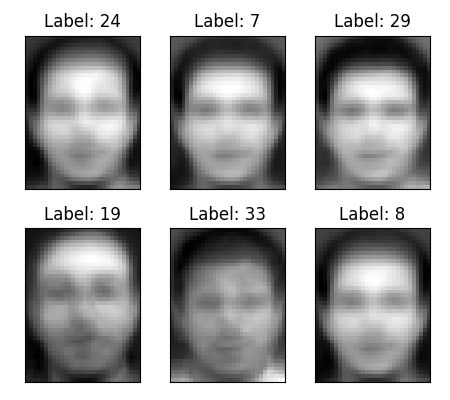
\includegraphics[width=0.7\columnwidth]{../source/orl/pictures/image-reconstructed-pca.png}
    \caption{ORL images reconstructed after PCA}
    \label{fig:orl-images-reconstructed}
\end{figure}

\begin{figure}[htbp]
    \centering
    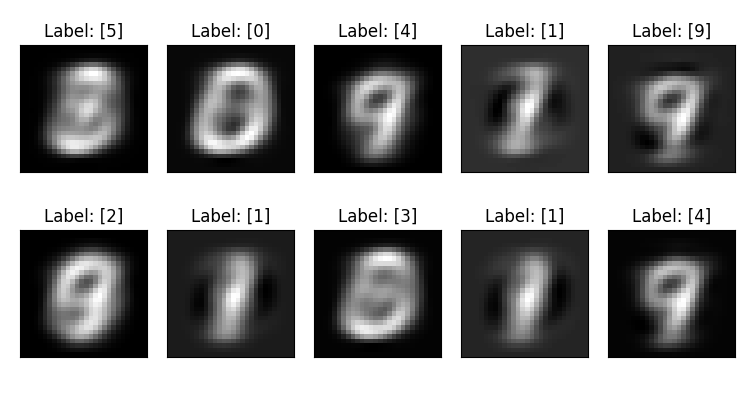
\includegraphics[width=0.7\columnwidth]{../source/mnist/pictures/image-reconstructed-pca.png}
    \caption{MNIST images reconstructed after PCA}
    \label{fig:mnist-images-reconstructed}
\end{figure}

Having the dimensions reduced to two, makes it easy to visualize the data. On Figure \ref{fig:mnist-scatter} can a scatter plot for the MNIST test data be seen. 

\begin{figure}[htbp]
    \centering
    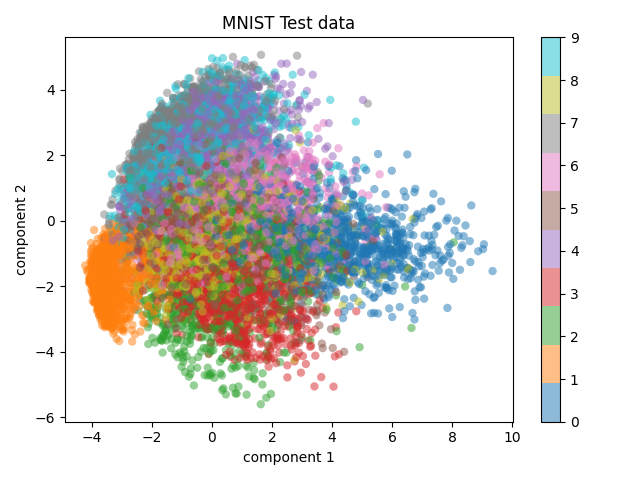
\includegraphics[width=1\columnwidth]{../source/mnist/pictures/mnist-scatter.png}
    \caption{MNIST test PCA images scatter plot}
    \label{fig:mnist-scatter}
\end{figure}

As for the ORL data set there is 40 classes, which is hard to illustrate in a single scatter plot. Therefore Figure \ref{fig:orl-scatter-first} contains the first 20 classes while Figure \ref{fig:orl-scatter-second} contains the other 20 classes. 


\begin{figure}[htbp]
    \centering
    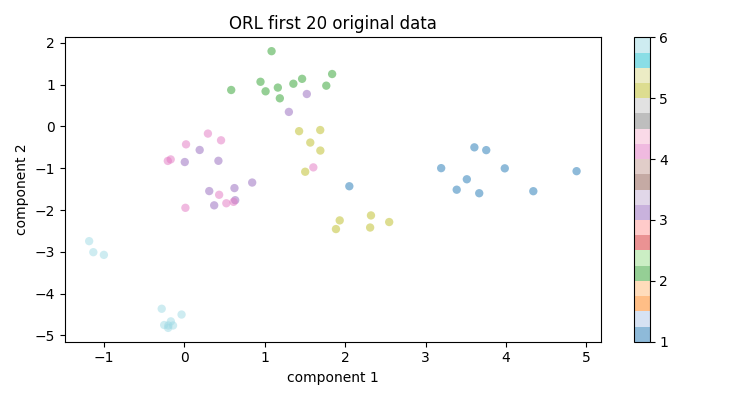
\includegraphics[width=1\columnwidth]{../source/orl/pictures/orl-scatter-original-first.png}
    \caption{ORL original PCA images first 20 classes}
    \label{fig:orl-scatter-first}
\end{figure}

\begin{figure}[htbp]
        \centering
        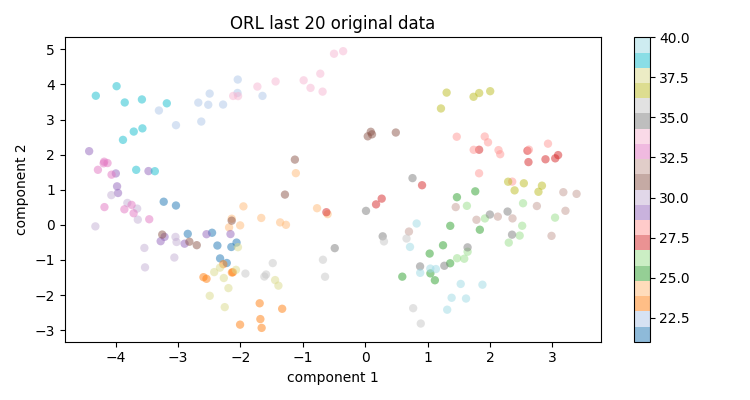
\includegraphics[width=1\columnwidth]{../source/orl/pictures/orl-scatter-original-second.png}
        \caption{ORL original PCA images last 20 classes}
        \label{fig:orl-scatter-second}
\end{figure}

\subsection{Classification}
Each classifier, for both the original data and the PCA version of the data, have their hyperparameters tuned if relevant. Afterwards the classification is performed.  
The accuracy of class predictions of the test data can be seen on Table \ref{tab:classifiers-performance}. Measurements of the time spent training can aswell be seen. 


\begin{table*}[!htbp]
    \centering
    \begin{tabular}{|l|l|l|l|l|l|} 
    \hline
    Dataset & Classifier                      & Accuracy (Raw)       & Accuracy (2d)        & Time (Raw)           & Time (2d)  \\ 
    \hline
    MNIST   & \multicolumn{1}{l}{}            & \multicolumn{1}{l}{} & \multicolumn{1}{l}{} & \multicolumn{1}{l}{} &            \\ 
    \hline
            & Nearest Class Centroid          & 82.03\%              & 43.65\%              & 0.702 s              & 0.016 s    \\ 
    \cline{2-6}
            & Nearest 2 Sub-Class Centroid    & 86.07\%              & 43.07\%              & 5.049 s              & 1.197 s    \\ 
    \cline{2-6}
            & Nearest 3 Sub-Class Centroid    & 88.24\%              & 42.39\%              & 7.918 s              & 1.918 s    \\ 
    \cline{2-6}
            & Nearest 5 Sub-Class Centroid    & 90.27\%              & 41.81\%              & 12.513 s             & 3.308 s    \\ 
    \cline{2-6}
            & Nearest Neighbor                & 96.88\%              & 42.43\%              & 14.173 s             & 0.207 s    \\ 
    \cline{2-6}
            & Perceptron with Backpropagation & 92.20\%              & 39.36\%              & 5.812 s              & 0.090 s    \\ 
    \cline{2-6}
            & Perceptron with MSE             & 86.08\%              & 32.79\%              & 5.923 s              & 0.128 s    \\ 
    \hline
    ORL     & \multicolumn{1}{l}{}            & \multicolumn{1}{l}{} & \multicolumn{1}{l}{} & \multicolumn{1}{l}{} &            \\ 
    \hline
            & Nearest Class Centroid          & 87.50\%              & 33.33\%              & 0.005 s              & 0.001 s    \\ 
    \cline{2-6}
            & Nearest 2 Sub-Class Centroid    & 94.17\%              & 40.00\%              & 0.602 s              & 0.548 s    \\ 
    \cline{2-6}
            & Nearest 3 Sub-Class Centroid    & 96.67\%              & 35.83\%              & 0.666 s              & 0.613 s    \\ 
    \cline{2-6}
            & Nearest 5 Sub-Class Centroid    & 96.67\%              & 34.17\%              & 0.828 s              & 0.748 s    \\ 
    \cline{2-6}
            & Nearest Neighbor                & 95.83\%              & 30.83\%              & 0.013 s              & 0.006 s    \\ 
    \cline{2-6}
            & Perceptron with Backpropagation & 95.83\%              & 13.33\%              & 0.073 s              & 0.015 s    \\ 
    \cline{2-6}
            & Perceptron with MSE             & 95.83\%              & 13.33\%              & 0.165 s              & 0.015 s    \\
    \hline
    \end{tabular}
    \caption{Performance of each classifier for both datasets}
    \label{tab:classifiers-performance}
\end{table*}

\subsection{Visualization}
Confusion matrices showing how certain classifiers performed when predicting labels for the test data can be seen on Figure \ref{fig:mnist-confusion} for the MNIST data set and on Figure \ref{fig:orl-confusion} for the ORL data set. 

\begin{figure*}[htbp]
        \begin{subfigure}[b]{.33\linewidth}
            \centering
            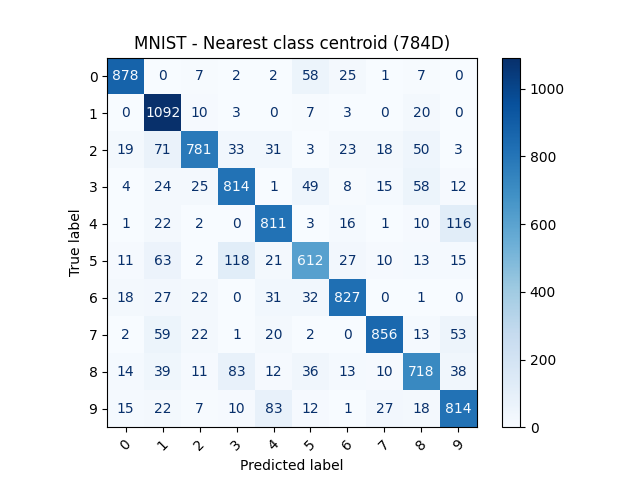
\includegraphics[width=1\linewidth]{../source/mnist/pictures/nearestClassCentroid-confusion-784d.png}
            \caption{Nearest class centroid (784D)}
            \label{fig:mnist-confusion-ncc-784}
        \end{subfigure}%
        \begin{subfigure}[b]{0.33\linewidth}
            \centering
            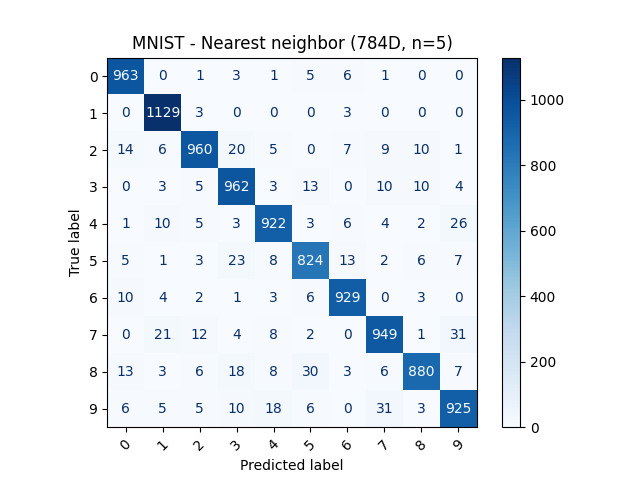
\includegraphics[width=1\linewidth]{../source/mnist/pictures/nearestNeighbor-5-confusion-784d.png}
            \caption{Nearest 5 neighbors (784D)}
            \label{fig:mnist-confusion-nn-784}
        \end{subfigure}
        \begin{subfigure}[b]{0.33\linewidth}
                \centering
                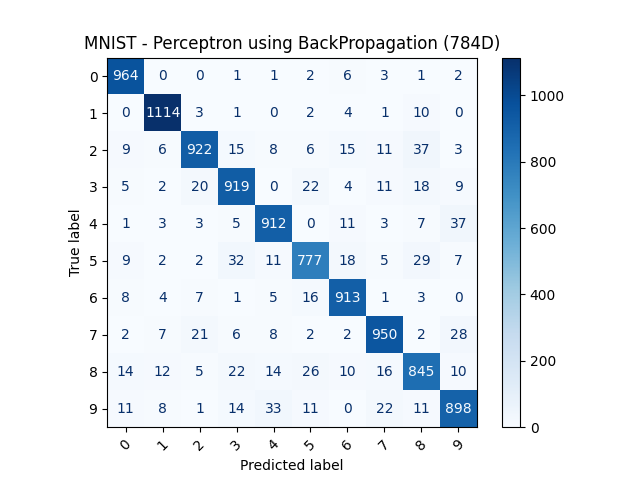
\includegraphics[width=1\linewidth]{../source/mnist/pictures/perceptronBP-confusion-784d.png}
                \caption{Perceptron using BP (784D)}
                \label{fig:mnist-confusion-pbp-784}
        \end{subfigure}

        \begin{subfigure}[b]{.33\linewidth}
                \centering
                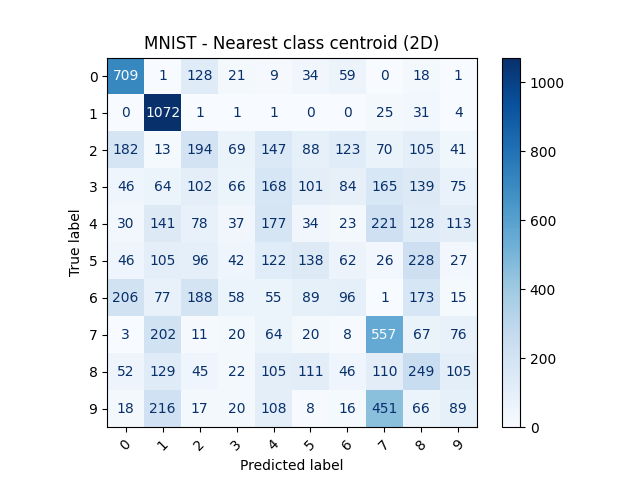
\includegraphics[width=1\linewidth]{../source/mnist/pictures/nearestClassCentroid-confusion-2d.png}
                \caption{Nearest class centroid (2D)}
                \label{fig:mnist-confusion-ncc-2}
            \end{subfigure}%
            \begin{subfigure}[b]{0.33\linewidth}
                \centering
                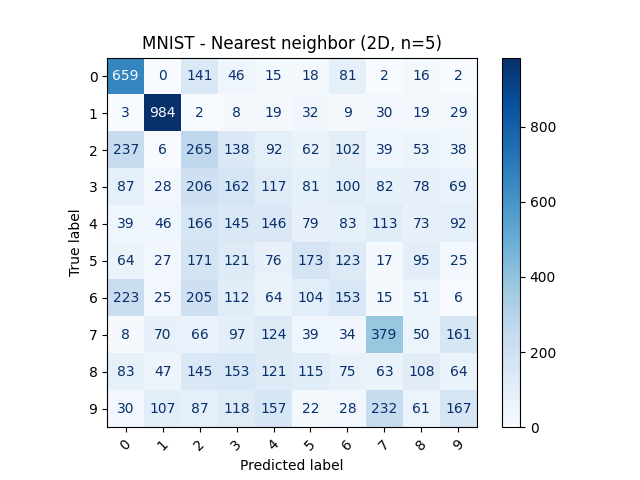
\includegraphics[width=1\linewidth]{../source/mnist/pictures/nearestNeighbor-5-confusion-2d.png}
                \caption{Nearest 5 neighbors (2D)}
                \label{fig:mnist-confusion-nn-2}
            \end{subfigure}
                \begin{subfigure}[b]{0.33\linewidth}
                    \centering
                    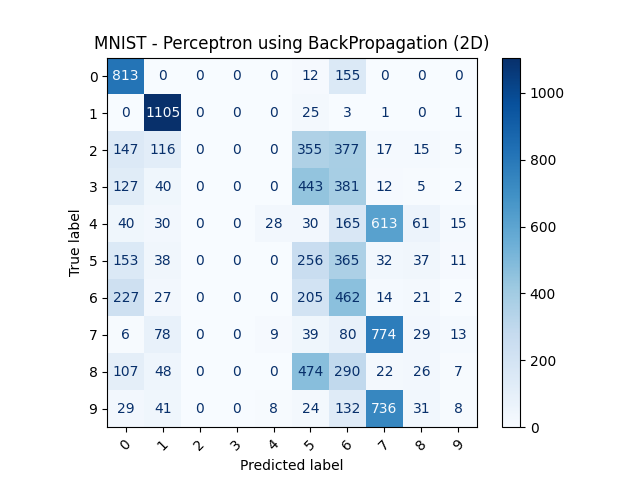
\includegraphics[width=1\linewidth]{../source/mnist/pictures/perceptronBP-confusion-2d.png}
                    \caption{Perceptron using BP (2D)}
                    \label{fig:mnist-confusion-pbp-2}
                \end{subfigure}
        \caption{Confusion Matrices - MNIST}
        \label{fig:mnist-confusion}
\end{figure*}
 
\begin{figure*}[htbp]
        \begin{subfigure}[b]{.33\linewidth}
            \centering
            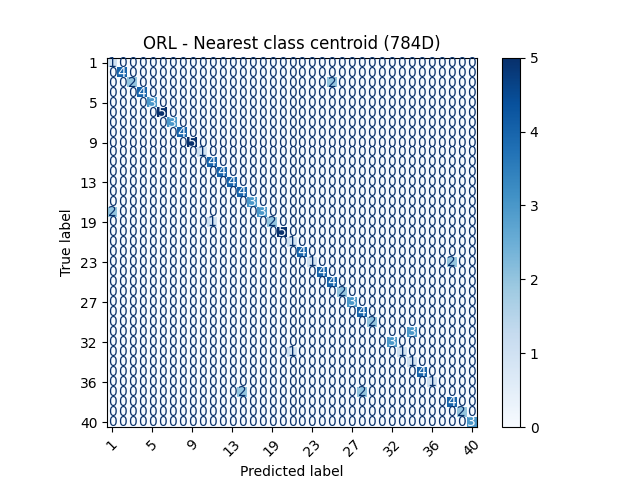
\includegraphics[width=1\linewidth]{../source/orl/pictures/nearestClassCentroid-confusion-784d.png}
            \caption{Nearest class centroid (784D)}
            \label{fig:orl-confusion-ncc-784}
        \end{subfigure}%
        \begin{subfigure}[b]{0.33\linewidth}
            \centering
            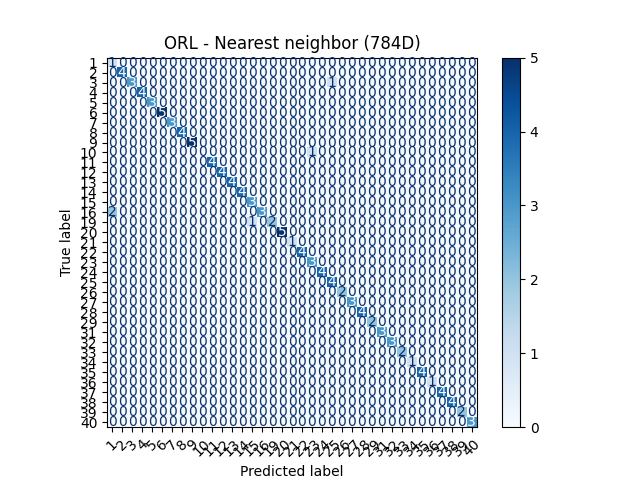
\includegraphics[width=1\linewidth]{../source/orl/pictures/nearestNeighbor-5-confusion-784d.png}
            \caption{Nearest 5 neighbors (784D)}
            \label{fig:orl-confusion-nn-784}
        \end{subfigure}
        \begin{subfigure}[b]{0.33\linewidth}
                \centering
                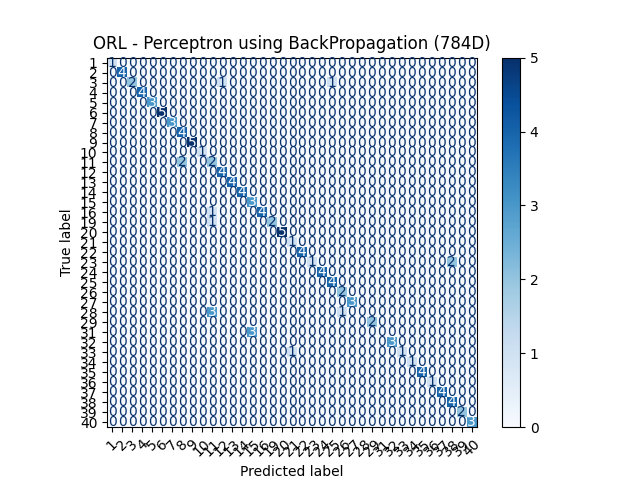
\includegraphics[width=1\linewidth]{../source/orl/pictures/perceptronBP-confusion-784d.png}
                \caption{Perceptron using BP (784D)}
                \label{fig:orl-confusion-pbp-784}
        \end{subfigure}

        \begin{subfigure}[b]{.33\linewidth}
                \centering
                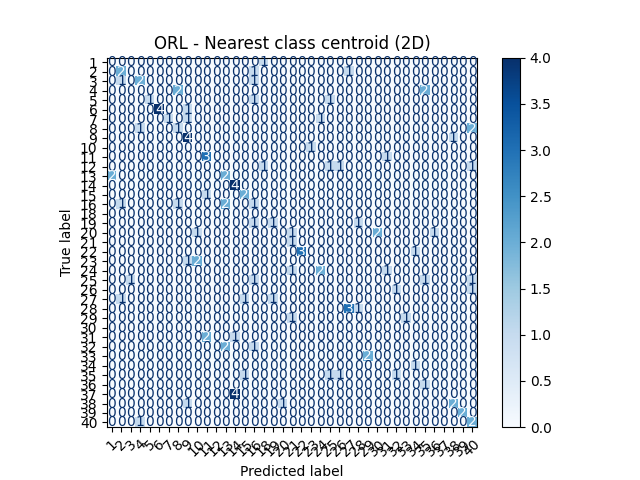
\includegraphics[width=1\linewidth]{../source/orl/pictures/nearestClassCentroid-confusion-2d.png}
                \caption{Nearest class centroid (2D)}
                \label{fig:orl-confusion-ncc-2}
        \end{subfigure}%
        \begin{subfigure}[b]{0.33\linewidth}
                \centering
                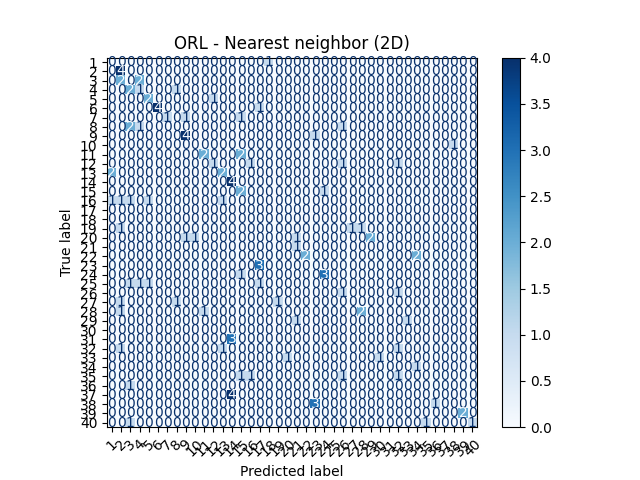
\includegraphics[width=1\linewidth]{../source/orl/pictures/nearestNeighbor-5-confusion-2d.png}
                \caption{Nearest 5 neighbors (2D)}
                \label{fig:orl-confusion-nn-2}
        \end{subfigure}
        \begin{subfigure}[b]{0.33\linewidth}
                \centering
                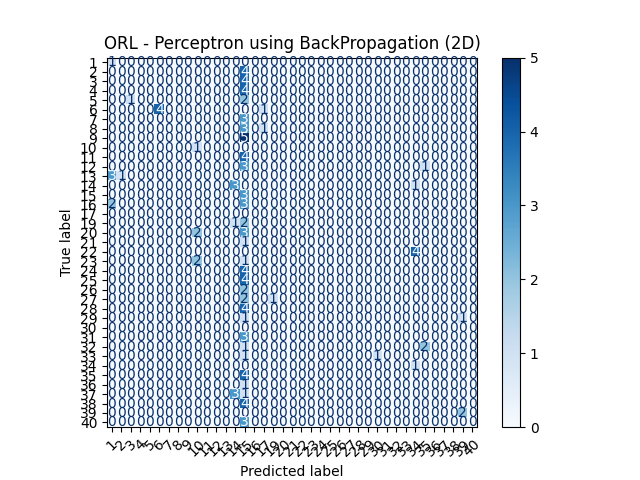
\includegraphics[width=1\linewidth]{../source/orl/pictures/perceptronBP-confusion-2d.png}
                \caption{Perceptron using BP (2D)}
                \label{fig:orl-confusion-pbp-2}
        \end{subfigure}
        \caption{Confusion Matrices - ORL}
        \label{fig:orl-confusion}
\end{figure*}

Scatter plot figures including boundary lines can be seen for certain classifiers on Figure \ref{fig:mnist-boundary-ncc}-\ref{fig:mnist-boundary-pbp}. The figures illustrates the class's boundaries for the trained models. 

\begin{figure}[htbp]
        \centering
        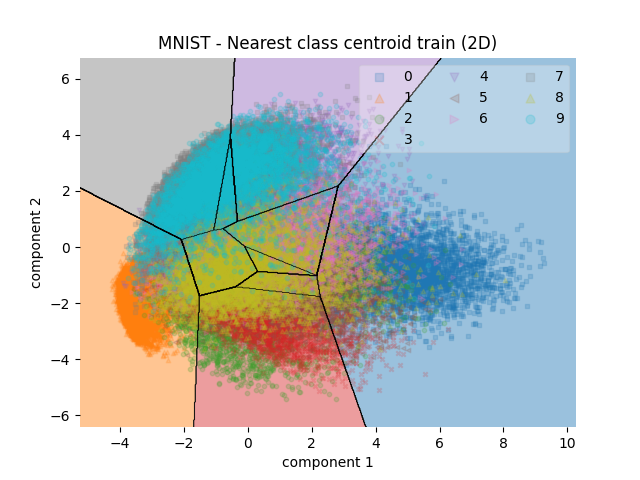
\includegraphics[width=1\columnwidth]{../source/mnist/pictures/nearestClassCentroid-boundary-train.png}
        \caption{Boundary Lines - Nearest Centroid train data}
        \label{fig:mnist-boundary-ncc}
\end{figure}

\begin{figure}
        \centering
        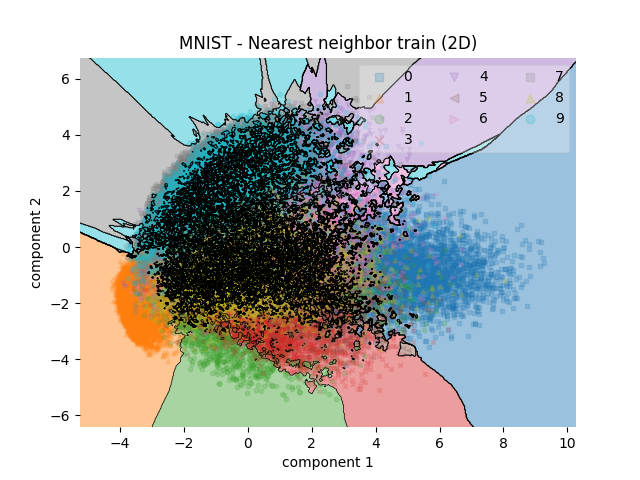
\includegraphics[width=1\columnwidth]{../source/mnist/pictures/nearestNeighbor-5-boundary-train.png}
        \caption{Boundary Lines - Nearest Neighbor train data}
        \label{fig:mnist-boundary-nn}
\end{figure}

\begin{figure}
        \centering
        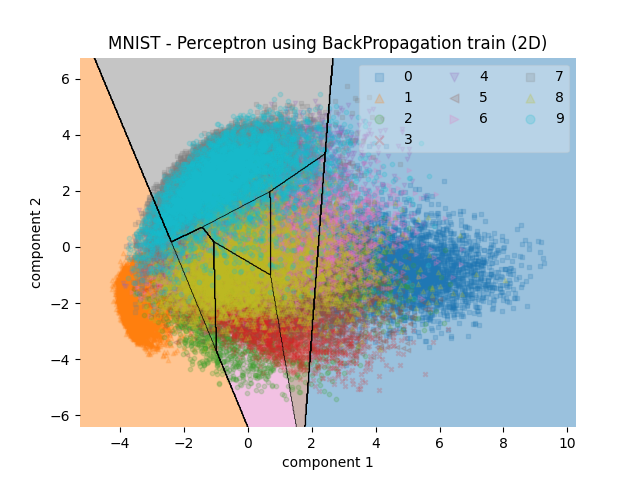
\includegraphics[width=1\columnwidth]{../source/mnist/pictures/perceptronBP-boundary-train.png}
        \caption{Boundary Lines - Perceptron using BP train data}
        \label{fig:mnist-boundary-pbp}
\end{figure}



\section{Discussion}
Comparing the performance of classification of the full features and to two features, it is clear that they distinguish. The accuracy is much lower using two features. As an example for Nearest Neighbor on the MNIST data set the accuracy for full features is 96.88\% while being 42.43\% on two features. Furthermore the training time is way faster on the lower features. Looking at the same example it takes 14.173 seconds to train the full features, but only 0.207 seconds on two features. It's seen on Figure \ref{fig:mnist-boundary-pbp} that there is only seven classes, meanwhile there is supposed to be ten. As shown in the confusion matrix on Figure \ref{fig:mnist-confusion-pbp-2} this clearly leads to test data being misclassified, where some classes are not represented at all. As PCA only looks into the variance of variables and not including response variables, it might have been better for the accuracy to utilize linear discriminant analysis instead. It's seen that the classifiers make different decision boundaries and vary in performance. For the MNIST data set Nearest Neighbor has the highest accuracy while being the slowest. Nearest 2 Sub-Class has the highest accuracy for both data sets with reduced features.           

\section{Conclusion}
\unfinished{Write conclusion}


\printbibliography
\end{document}